\chapter{Performance}
We will now look at how the different languages compare in
performance. We will start by taking a brief look at which
optimisations are implemented in each language, and what we can expect.

\section{Optimisations}

\subsection{Deforestation}
Stream fusion, program composition or deforestation is a technique
that aims composing several functions into one to optimize away
intermediate datastructures\footnote{which it what gives it the name
  deforestation: intermediate tree structures are removed} and thus
avoid expensive memory access.

A simple example is that of computing sum of squares:
\begin{verbatim}
foldl (+) 0 (map (^2) xs)
\end{verbatim}
where the unoptimized program would have to write all the squared
numbers into memory during the computation of map and then read back
from memory during the summation. Fusing the \verb|map| into the
\verb|foldl| avoids this intermediate array:
\begin{verbatim}
foldl (\a b -> a + b^2) 0 xs
\end{verbatim}

This optimization is at the heart of both the Nikola and Repa
architectures, where it happens through the use of delayed
arrays. Data.Vector also performs some stream fusion by employing GHC
rewrite rules. Fusion is currently being implemented in
Accelerate. The newest version on Hackage (0.12.1.0) does not perform
any fusion, but the development repository contains a not completely
functional implementation, so it will possibly be part of the next
release.

On GPU hardware this also means that several kernels can be merged
into one, and the overhead involved in kernel launches can thus also
be avoided.

In CUDA this optimization must be done by hand \todo{Cite someone that
  says nvcc doesn't provide deforestation/fusion}

\subsection{Prefix sum, tree reduction}
Accelerate comes with a number of built in parallel algorithms, that
runs efficiently on GPUs. Such as

\subsection{Strided memory access}
Because of limited caches in GPUs, out of order memory access incurs a
huge performance penalty. We must thus make sure that memory accesses
inside GPU warps are coalesced.

Accelerate guarantees this approach, as long as you use the built in
high order functions, and avoid using the array lookup function
\begin{verbatim}
(!) :: (Shape ix, Elt e) => Acc (Array ix e) -> Exp ix -> Exp e
\end{verbatim}

\todo{Nikola??} 

\subsection{Limit branch divergence}
Accelerate goes a long way to restrict the possible programs you can
write, such that they can make certain performance guarantees. For
instance, they do not allow you to write sequential loops running on
the GPU as this may allow one thread to diverge letting the remaining
threads in a block waiting. This is problematic, as certain problems
are more efficiently expressed using nested loops, and you thus need
to manually flatten, giving a performance penalty.

Nikola on the other hand, does not make such limitations and lets the
programmer himself evaluate \todo{complete this}

\section{Benchmark setup}

\subsection{Hardware}
All benchmarks have been performed on a computer provided by the
HIPERFIT research center running Ubuntu 12.04 LTS and CUDA 5.0.

The hardware specifications is as follows:

\begin{itemize}
\item 2 $\times$ AMD Opteron\texttrademark\ 6274 processors (16 cores each, clocked at 2,2 Ghz)
\item 125-132 GB of main memory \todo{What is the real value here? /proc/meminfo says 125 GB - but an odd number?}
\item Quad SLI consisting of two GeForce GTX 690 (each a dual-head GPU). See full specifications in Table \ref{tab:hardware}.
\end{itemize}

\begin{table}
  \centering
  \begin{tabular}{ll}
    Memory & $2 \times 2048$ MiB \\
    Multiprocessors & $2 \times 8$ SMs\\
    Cores per SM & 192 cores \\
    CUDA cores & $2 \times 1536$ cores\\
    Clock rate & 915 Mhz \\
    RAM technology & GDDR5 \\
    Memory bandwidth & $2 \times 192.3$ GB/s \\
    \hline
  \end{tabular}
  \caption{Geforce GTX 690 specification}
  \label{tab:hardware}
\end{table}

% Ideally we would have evaluated all benchmarks on two different GPUs,
% to make sure we were not optimizing for the behavior of a single
% unit. We did however only have access to this machine with CUDA
% version >= 4.0 (which was a requirement for \todo{Was it Nikola,
%   Accelerate or both?}. The other machine we have access to only
% provides CUDA 3.2.

\subsection{Software and compilation}
\todo{Introduce our suite of survey tools, how execution time are
measured, criterion, Individual GHC installations for each library}


% \subsection{Benchmark setup}
% Several of the libraries we have tested requires individual
% compilation steps before the actual computation can take place. We
% have decided not to include all initialization in the running times,
% and only record the time used on the actual computation and eventual
% memory allocation and transfers. This is done to make the comparison
% fair, and because we think it is more important to optimize the actual
% computation. Optimizing the compilation or interpretation performance
% is also important, but we find that to be less of priority now and it
% thus out of our current scope.


\section{Benchmarks}
We will now present the results of our benchmarks. We have two plots
for each benchmark: One showing the actual time used on each
computation, and one showing relative performances.

\begin{figure}
	\centering
\begin{adjustbox}{minipage=1.3\textwidth,margin=0pt \smallskipamount,center}
	\subbottom[]{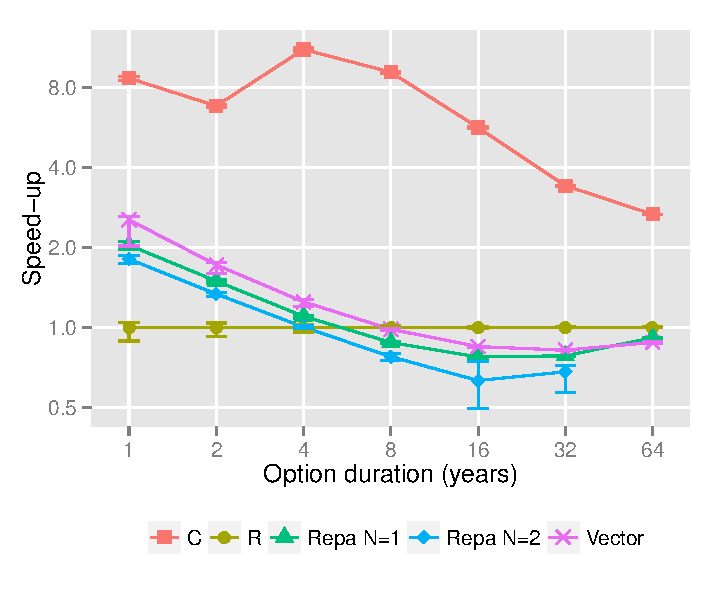
\includegraphics[width=0.5\textwidth]{graphics/final-benchmark/binomial-cpu/speedup-graph.pdf}\label{fig:binomial-cpu-speedup}}
	\subbottom[]{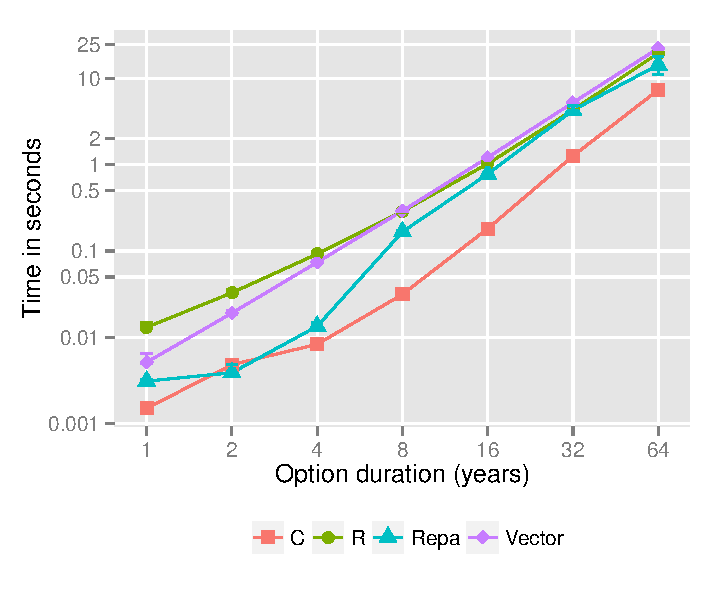
\includegraphics[width=0.5\textwidth]{graphics/final-benchmark/binomial-cpu/time-graph.pdf}\label{fig:binomial-cpu-time}}
\end{adjustbox}
  \caption{\textbf{(a)}  \textbf{(b)} }
\label{fig:binomial-cpu}
\end{figure}

\begin{figure}
	\centering
\begin{adjustbox}{minipage=1.3\textwidth,margin=0pt \smallskipamount,center}
	\subbottom[]{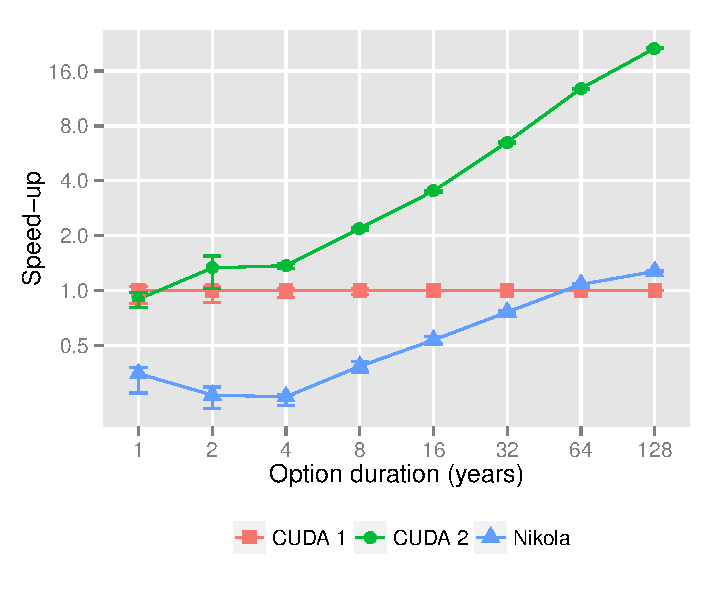
\includegraphics[width=0.5\textwidth]{graphics/final-benchmark/binomial-gpu/speedup-graph.pdf}\label{fig:binomial-gpu-speedup}}
	\subbottom[]{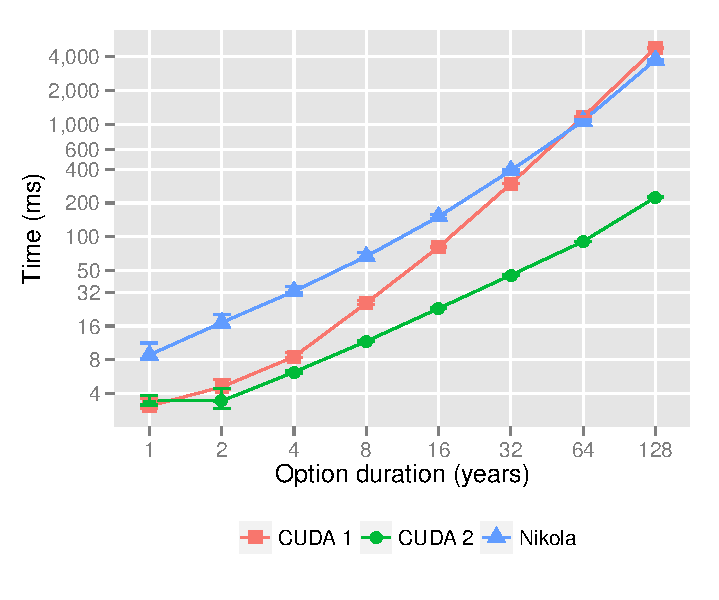
\includegraphics[width=0.5\textwidth]{graphics/final-benchmark/binomial-gpu/time-graph.pdf}\label{fig:binomial-gpu-time}}
\end{adjustbox}
  \caption{\textbf{(a)}  \textbf{(b)} }
\label{fig:binomial-gpu}
\end{figure}

\begin{figure}
	\centering
  \begin{adjustbox}{minipage=1.3\textwidth,margin=0pt \smallskipamount,center}
	\subbottom[]{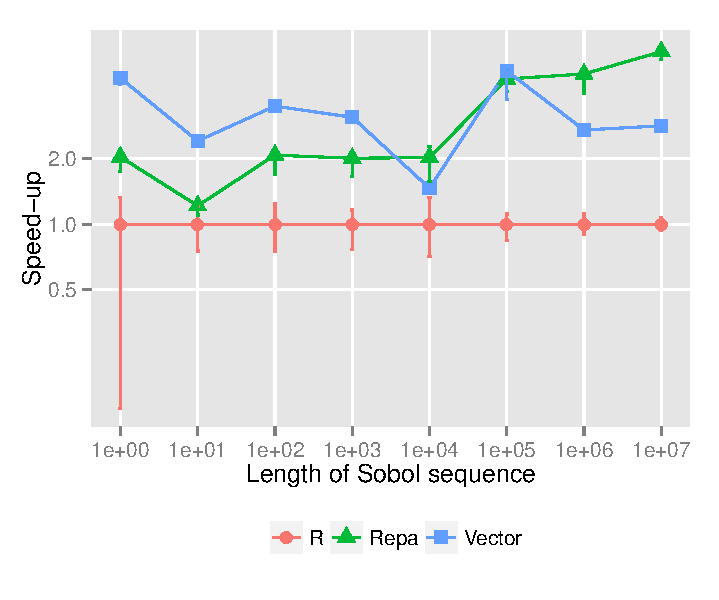
\includegraphics[width=0.5\textwidth]{graphics/final-benchmark/sobol-cpu/speedup-graph.pdf}\label{fig:sobol-cpu-speedup}}
	\subbottom[]{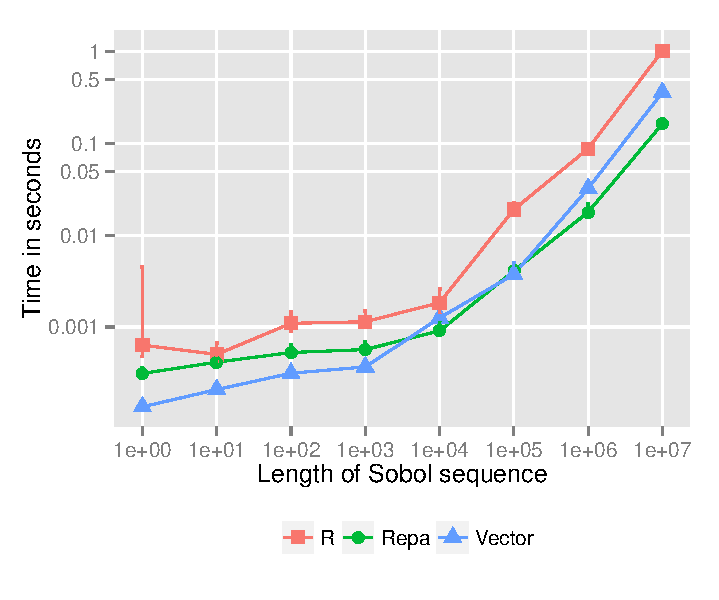
\includegraphics[width=0.5\textwidth]{graphics/final-benchmark/sobol-cpu/time-graph.pdf}\label{fig:sobol-cpu-time}}
\end{adjustbox}  
  \caption{\textbf{(a)}  \textbf{(b)} }
\label{fig:sobol-cpu}
\end{figure}

\begin{figure}
	\centering
\begin{adjustbox}{minipage=1.3\textwidth,margin=0pt \smallskipamount,center}
	\subbottom[]{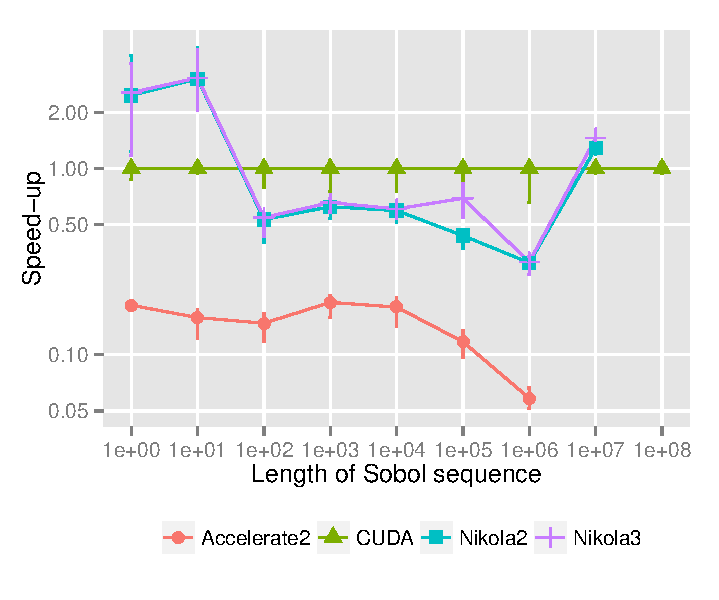
\includegraphics[width=0.5\textwidth]{graphics/final-benchmark/sobol-gpu/speedup-graph.pdf}\label{fig:sobol-gpu-speedup}}
	\subbottom[]{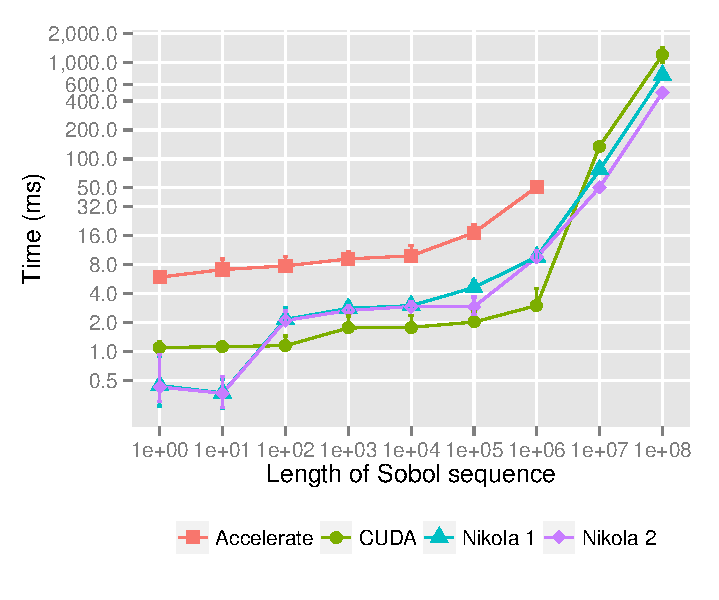
\includegraphics[width=0.5\textwidth]{graphics/final-benchmark/sobol-gpu/time-graph.pdf}\label{fig:sobol-gpu-time}}
\end{adjustbox}
  \caption{\textbf{(a)}  \textbf{(b)} }
\label{fig:sobol-gpu}
\end{figure}

\begin{figure}
	\centering
\begin{adjustbox}{minipage=1.3\textwidth,margin=0pt \smallskipamount,center}
	\subbottom[]{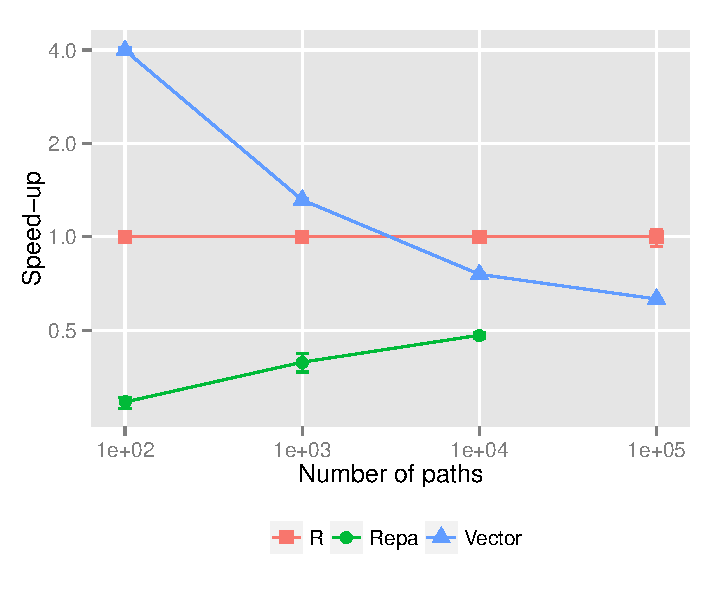
\includegraphics[width=0.5\textwidth]{graphics/final-benchmark/lsm-cpu/speedup-graph.pdf}\label{fig:lsm-cpu-speedup}}
	\subbottom[]{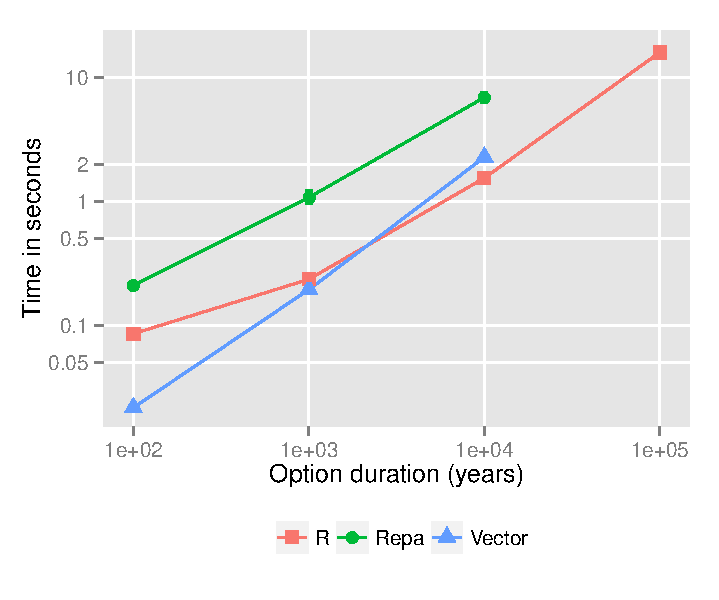
\includegraphics[width=0.5\textwidth]{graphics/final-benchmark/lsm-cpu/time-graph.pdf}\label{fig:lsm-cpu-time}}
\end{adjustbox}
  \caption{\textbf{(a)}  \textbf{(b)} }
\label{fig:lsm-cpu}
\end{figure}




% Speed up graph. In the graph we use the sequential version written
% with Data.Vector as a baseline for the comparison.

% Accelerate is not included, because of problems in their stream fusion
% algorithm leading to running times that evolve
% exponentially. Disabling fusion lead to CUDA exceptions.

% We see that the overhead incurred by using Nikola makes both
% sequential implementations (R and Data.Vector) faster for the smallest
% cases, and only when we reach the largest example (128 years expiry
% time) Nikola catches up.

% Repa is the best performing, even though it does not perform any GPU
% computations. We are not sure why Repa gives so varied speed-ups for
% different input sizes, but it might be because of our somewhat
% arbitrary threshold for which problem sizes should be executed in
% parallel and which should be executed sequentially.


%%% Local Variables:
%%% mode: latex
%%% TeX-master: "../master"
%%% End:
